\begin{DensePanel}{250mm}{10}{REACH AND TRANSFER}
  \noindent\begin{minipage}[t]{186mm}\vspace{0pt}
    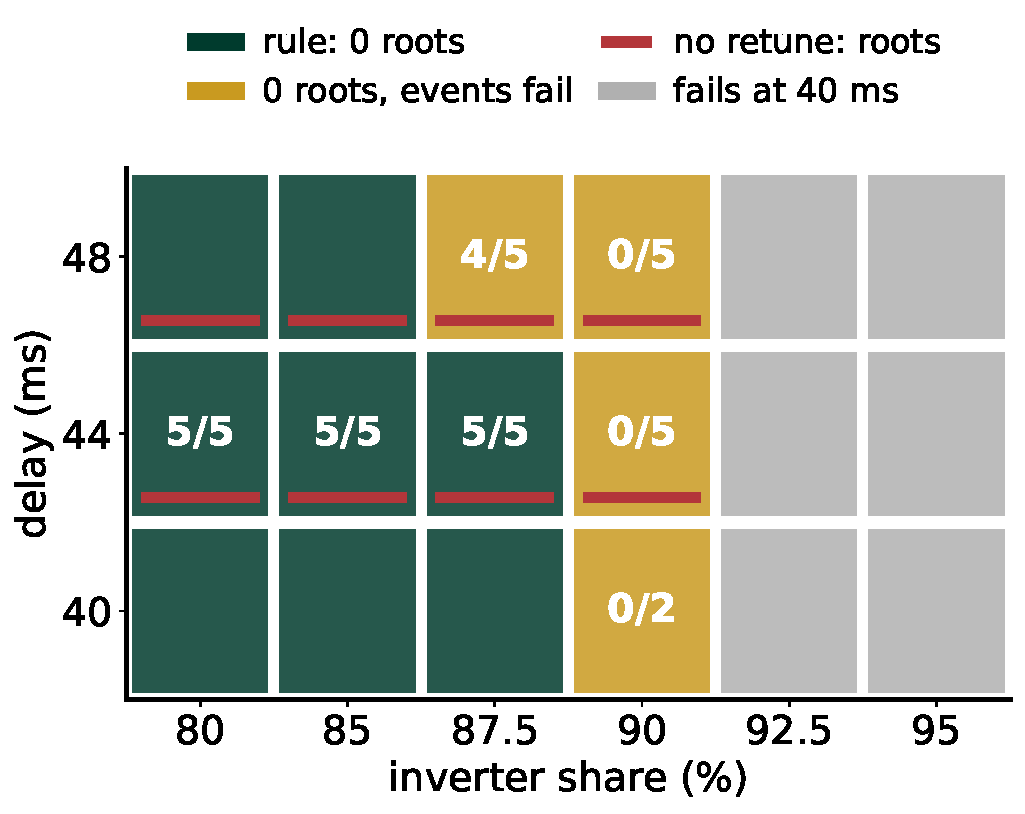
\includegraphics[width=184mm,height=118mm,keepaspectratio]{generated/figures/share_delay_map.pdf}
  \end{minipage}\hfill%
  \begin{minipage}[t]{86mm}\vspace{2mm}
    {\DenseSmall Each cell: roots beyond the margin with the rule; red bar: same cell, no retune; numbers: events passed.\par}
  \end{minipage}\par
  \vspace{1mm}
  \begin{DenseWords}\textbf{\color{IASGold!65!black}IN WORDS\ \ }The rule extends delay tolerance at every share where 40 ms is feasible. It does not raise the maximum share: at 90\,\% even the 40 ms design fails the events (0 of 2); 92.5\,\% fails at 40 ms.\end{DenseWords}
  \vspace{2mm}
  {\DenseSmall \textbf{Second design} (85\,\%), rule applied unchanged: 0 roots, \textbf{5 of 5} events. \textbf{Nine-bus bank} (assumed data): $+0.886\to-0.131\ \mathrm{s^{-1}}$, re-run. \textbf{First-order formula}: same counts; the choice of mode matters, not the truncation.\par}
\end{DensePanel}
